\documentclass[11pt]{article}
\usepackage[margin=1in]{geometry}
\usepackage{graphicx}
\usepackage{hyperref}
\usepackage{amsmath}

\graphicspath{{./Figures/}}

\begin{document}

\title{Asynchronous I/O for \texttt{cp -r}}
\date{\today}
\author{Vincent Lee \\
        Gualberto A. Guzman}

\maketitle

\section{Goals} \label{sec:goals}

Our project proposal is to use Linux's asynchronous IO interfaces (aio) to build
an optimized version of \texttt{cp -r}. We intend to demonstrate differences in
the effects of caching, readahead, and other factors on aio performance,
especially as they relate to SSDs vs HDDs. Our implementation takes an existing
directory name and a new name and copies the entire directory tree to the
location specified. We achieve competitive results within 1.5x the speed of
native \texttt{cp -r}.

\section{Major Decisions} \label{sec:maj_dec}

There were two major choices available to us for asynchronous file IO on Linux.
The first was the \textbf{POSIX AIO} interface, which is standardized as a set
of library calls across all POSIX-compliant environments. However, according to
the man pages, \texttt{glibc} simulates \textbf{POSIX AIO} completely in
userspace~\cite{aio7}. This means that the kernel is not able to make scheduling
and reordering decisions that may affect performance. Instead, we decided to use
the nonportable \textbf{Linux AIO} system calls.

For the implementation itself, \textbf{C++} was chosen as the programming
language. In addition to being a fast systems programming language, it also
provides useful abstractions and standard libraries, as well as access to the
Boost libraries. The Boost Filesystem library was used for its
\texttt{recursive\_directory\_iterator}, an iterator which yields all paths
along a breadth-first traversal from a given root path. For each path, if the
file is small enough, it is copied directly using a Boost call. This is because,
below a certain point, the overhead of initializing and submitting an
asynchronous IO task dominates the cost of simply using \texttt{read} and
\texttt{write}. This threshold is configurable and the effects of varying it are
explored in section~\ref{sec:eval}.

\section{Implementation} \label{sec:impl}

After parsing all arguments, \texttt{acpr} initializes a recursive directory
iterator from Boost, which yields a breadth-first traversal of every path in the
given source directory. For each path, we run \texttt{lstat} to discover if it
is a file or directory. If a directory, we create it immediately in the output
path with \texttt{mkdir}. Since the iterator is breadth-first, we are guaranteed
that all parent directories exist at the time of calling. If a file and it is
below the AIO threshold, we copy it using a Boost utility function,
\texttt{boost::filesystem::copy\_file}, implemented with \texttt{read} and
\texttt{write}. Otherwise, we use the AIO system.

\subsection{AIO Copying} \label{sec:aio_copy}

A copy of a single file using AIO is represented by a class \texttt{CopyTask}.
This class encapsulates the state of each copy, as well as a fixed number of
\texttt{iocb}'s. An \texttt{iocb} is the AIO system's unit of work. Each time
\texttt{CopyTask::schedule\_next\_read} is called, we scan to see if there are
any free \texttt{iocb}'s, and attach to each of them offsets to read, the file
descriptor to read from, a buffer to read into, and a callback to invoke when
complete. Once enough \texttt{iocb}'s have been buffered, the system call
\texttt{io\_submit} is invoked, passing all initialized \texttt{iocb}'s to the
kernel. 

At the end of each loop of the recursive directory iterator, another system
call, \texttt{io\_getevents}, is called to gather any completed reads and writes
from the kernel and invoke their callbacks. This call takes a timeout that
represents the maximum time the user is willing to wait for the kernel to give
it events. Whenever a callback for a write is invoked, it invokes
\texttt{CopyTask::schedule\_next\_read}. The \texttt{CopyTask} corresponding to
each \texttt{iocb} is kept in a private lookup table, enabling it to be
recovered from the callbacks, which are global function pointers. Whenever a
callback for a read is invoked, it simply reinitializes the \texttt{iocb} into a
write, changes the file descriptor to the output file, and immediately resubmits
it. Here, we potentially could have performed batching of writes to reduce the
number of system calls, but due to complexity concerns and time limits, decided
to leave it as-is although it is a issue for future work.

After the directory iterator finishes, the event queue is then drained by
calling \texttt{io\_getevents} in a loop with unlimited timeout until the
\texttt{iocb} to \texttt{CopyTask} lookup table is empty, meaning all
\texttt{CopyTask}s have completed.

\section{Challenges and Limitations} \label{sec:challenge}

Our first challenge was dealing with the lack of proper documentation for the
Linux AIO API. The user space library was poorly documented in general and has
not been updated since 2015; we had to find an Ubuntu man page from 2012 in
order to see examples of its usage~\cite{ubuntu}. 

Secondly, A function critical to our implementation,
\texttt{boost::filesystem::relativize}, was missing in the version of Boost
installed on the lab computers (1.58). This function takes two absolute paths
and makes one into a path relative to the other, so that it can be appended to
the destination directory. We backported this function from a later Boost
version (1.60) by simply copying the relatively small implementation (160 lines)
from the Boost source control~\cite{boost}.

In addition, the userspace header library that wrapped the Linux AIO system also
implemented a particular call na\"ively. \texttt{io\_queue\_run} is a function
that polls the kernel event queues and runs callbacks. However, we looked at the
implementation and discovered that it was receiving events one by one, making a
separate system call for every single one. We replaced calls to this function
with direct system calls to read the event queue ourselves, reducing the amount
of system calls needed to process the same number of events. 

During early testing, we attempted to copy the Linux 4.4.97 kernel tree on an
SSD, a 711 megabyte repository of mostly small files. \texttt{acpr} used over 7
minutes before it was killed, while \texttt{cp -r} used only 1 second. Some
profiling indicated that the AIO subsystem finished very quickly, it was the
\texttt{fsync} call for each file that slowed everything down. Disabling the
\texttt{fsync} by default sped the copy up to about 3 seconds. We later verified
that \texttt{cp} also chose not to call it by observing the system calls it made
using \texttt{strace}. 

Currently, attributes and ownership are not completely copied from the source to
the destination. In addition, due to complications arising from relative
symbolic links, all symbolic links are skipped when copying.

The event queue is processed with the single calling thread. A potential
optimization would have been to have a separate thread driving the event queue
while the main thread iterates the directory, but for simplicity, \texttt{acpr}
is limited to a single-thread implementation.

\section{Evaluation} \label{sec:eval}

\texttt{acpr} was evaluated on two main platforms types, two laptops running
Linux with an SSD, and a csres server machine. The test script first runs
\texttt{cp -r} on the directories under test, then runs \texttt{acpr} to another
destination directory, and times both. The test script also has the ability to
sync and clear the buffer cache by calling \texttt{echo 3 >
/proc/sys/vm/drop\_caches}, which we opt to do for almost all cases below, to
test the AIO system's ability to reorder requests effectively for IO. After
copying, the source and destination directories were compared using
\texttt{diff -r}, which performs a deep diff of the entire subtree to find
corrupt, absent, or extra files from the copy.

We test two major cases, copying a large file (Lubuntu ISO, 880MB) and copying
the Linux 4.4.97 (771MB) source tree. The first exercises \texttt{acpr}'s
ability to fully utilize the disk's speed, while the second emulates real-world
scenarios of copying subtrees filled with files of varying sizes. In all cases,
we average completion time in seconds over ten trials on a relative noise-free
machine. We note, however, that since the Linux kernel contains some relative
symlinks, which we skip, the test script's error-checking will report
differences. We have manually verified using \texttt{diff -r} that \texttt{acpr}
is copying the output correctly. 

\subsection{Thinkpad X1 Carbon \& Macbook Pro} \label{subsec:laptops}

The first laptop is a 2013 Thinkpad X1 Carbon, with Arch Linux, updated to the
latest packages as of December 5, 2017. The laptop has an Intel i7-4600U
processor clocked at 2.1 GHz, 8 GB of RAM, and 4 GB of swap space configured.
The tests were run on the owner's home directory, which is on a local ext4
partition on a Samsung MZNTD256 SSD. The second laptop in a Mid-2015 Macbook Pro
(version 11,5) running Ubuntu Linux 16.04.2. It has a 2.5 GHz Intel Core
i7-4870HQ, 16GB of RAM, and 4GB of swap space. As in the first case, all tests
were run on the owner's home directory, on a local ex4 partition on an Apple
SM0512G SSD.

\subsubsection{Copying a Single Large File} \label{ssubsec:laptops_large}

\begin{figure}[ht!]
        \begin{minipage}{.33\textwidth}
                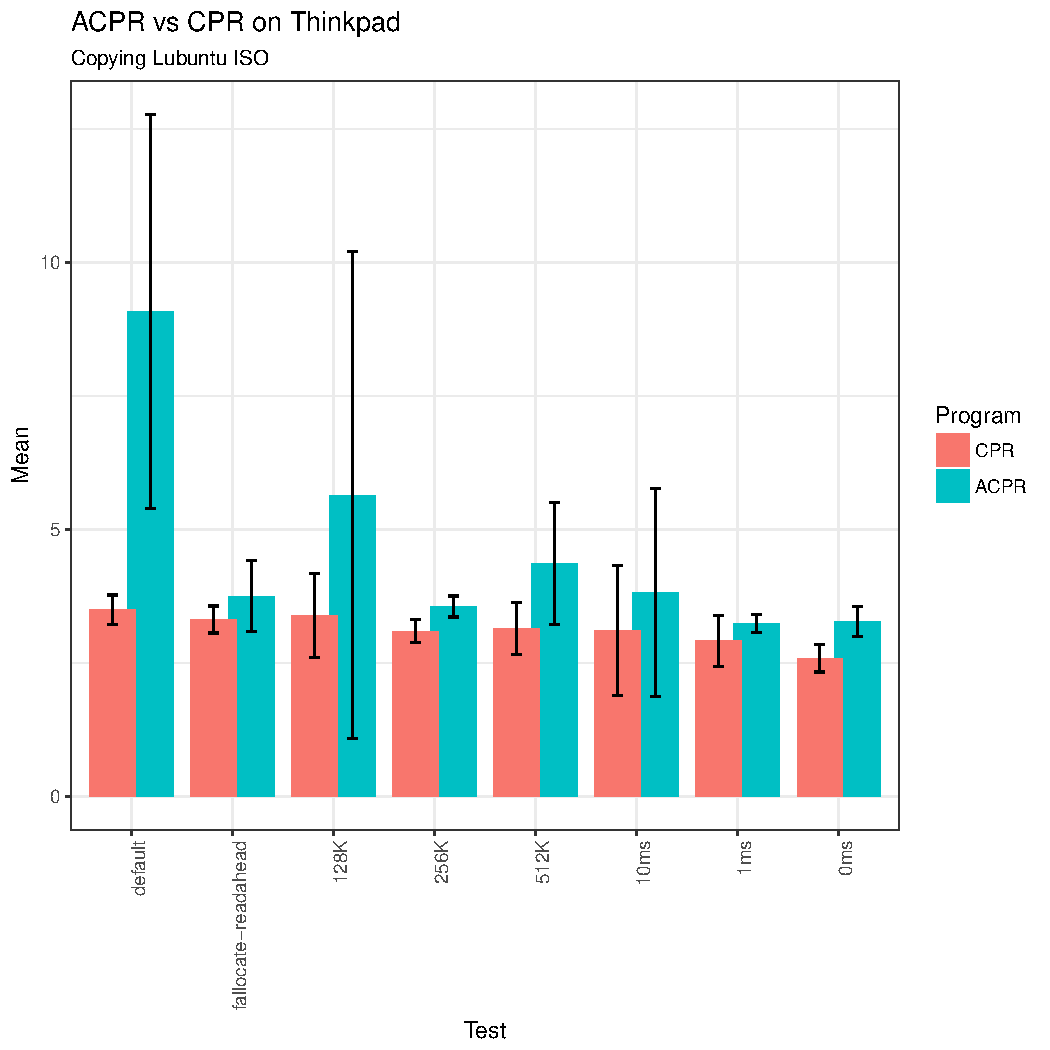
\includegraphics[width=1.8\textwidth,]{Laptop_Lubuntu_Barplot.pdf}
                \caption{Copying Lubuntu on Thinkpad}
                \label{fig:laptop_lubuntu}
        \end{minipage}
        \hspace{3cm}
        \begin{minipage}{.33\textwidth}
                \centering
                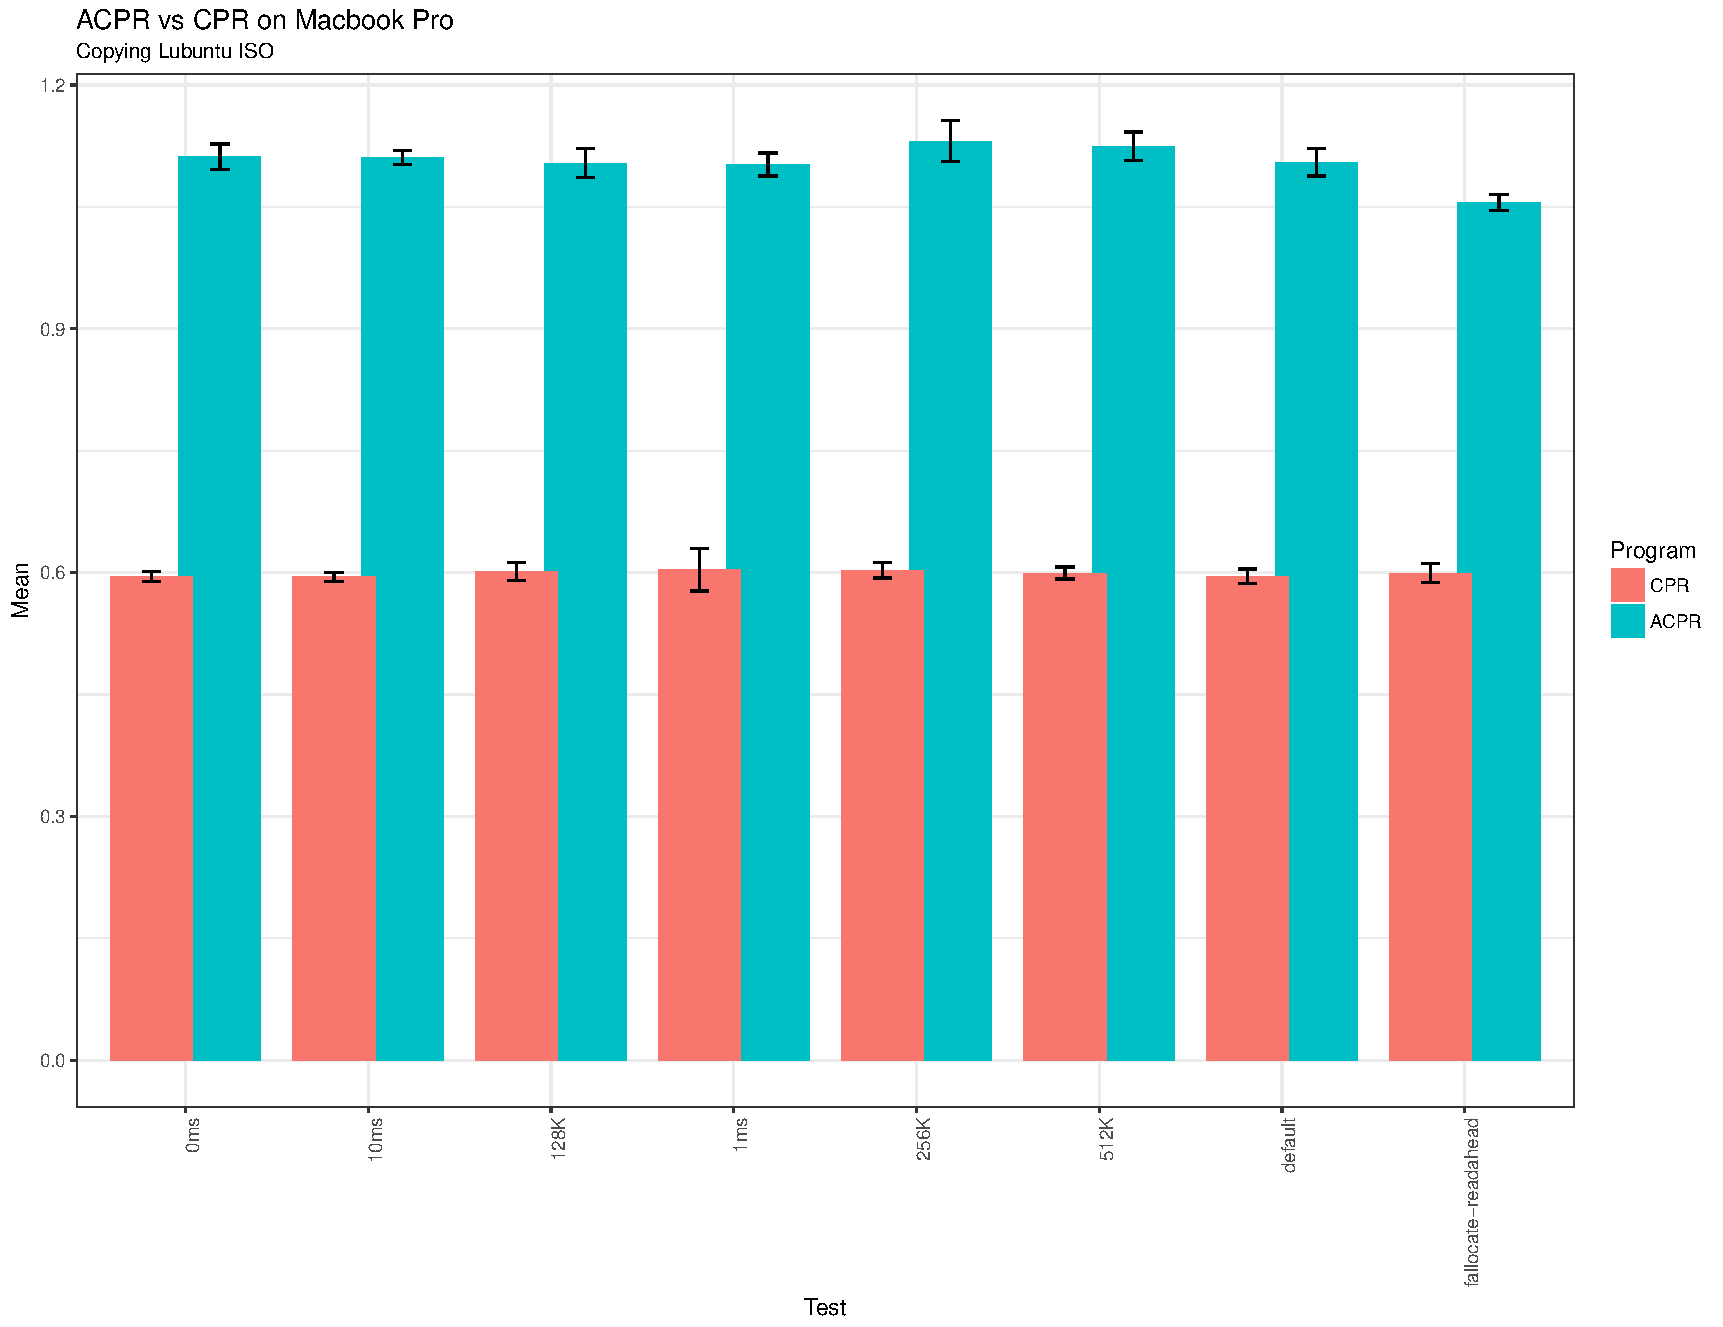
\includegraphics[width=1.8\textwidth,]{Macbook_Lubuntu_Barplot.pdf}
                \caption{Copying Lubuntu on Macbook Pro}
                \label{fig:macbook_lubuntu}
        \end{minipage}
\end{figure}

First, we compare a run of \texttt{acpr} with all default options with
\texttt{cp -r} in Figure~\ref{fig:laptop_lubuntu} and
Figure~\ref{fig:macbook_lubuntu}. For the Thinkpad, \texttt{cp -r} copies the
ISO in about 3.5 seconds on average, coming to an average of 251 MB/s
throughput. \texttt{acpr} is weaker, copying the ISO in about 9 seconds, coming
to an average of 96.9 MB/s throughput.  However, if \texttt{acpr} calls
\texttt{fallocate} to preallocate the destination file and \texttt{readahead} on
the source file, then it can copy the ISO in 3.75 seconds, a throughput of 234.6
MB/s. For the Macbook Pro, \texttt{cp -r} copies the ISO in about 600 ms, coming
to an average of 1478 MB/s throughput. In this case, calling \texttt{fallocate}
and \texttt{readahead} does not improve performance much beyond 1.1s with a
throughput of 833 MB/s. In comparison to the Thinkpad, the Macbook Pro benefits
greatly from the increased bus speed as shown by the tighter errors bars in each
case. However, in both cases we cannot improve beyond native \texttt{cp -r}
performance. This is likely because the AIO system is more indirect, and the
system is perhaps unable to detect that a sequential read is occurring, unlike
\texttt{cp -r} where the repeated calls to \texttt{read} and \texttt{write} make
it very clear that a sequential copy is occurring.

Next, we run the copy with larger block sizes. By default, \texttt{acpr} copies
64K per AIO operation. Increasing the size may not make much difference if the
files are smaller than 64K anyway, but should decrease the number of system
calls and improve locality of the buffers when copying a single large file. When
increasing the block size to 128K on the Thinkpad, runtime decreases from the
baseline of 9 seconds to 5.64 seconds and a throughput of 155.9 MB/s. Further
increasing the block size to 256K again improves the performance to 3.55s and
247.6 MB/s. However, increasing again to 512K yields a performance drop to 4.35s
and 201.9 MB/s as seen in Figure~\ref{fig:laptop_lubuntu}. On the Macbook Pro,
increasing the block size beyond the default of 1.1s and 769 MB/s throughput
results in a performance decrease of 1.13 s and 782 MB/s throughput. As shown in
Figure~\ref{fig:macbook_lubuntu}, the small variation in results from varying
the block size do not indicate a concrete performance gain. This is probably due
to overhead allocating and copying such large buffers across the user-kernel
boundary.

Finally, we test what happens if we vary the timeout when gathering events. By
default, \texttt{acpr} allows the kernel 5 ms to respond with events, yielding
the baseline measurement of 9 seconds and 96.9 MB/s. Increasing this timeout to
10 ms improves performance to 3.81 seconds and 230.9 MB/s, while decreasing it
to 1 ms also improves performance in a similar manner to 3.23 seconds and 272.4
MB/s for the Thinkpad. Eliminating the timeout (passing 0 to the kernel) also
gives a similar boost to 3.26s and 269.2 MB/s. The effect is similarly
negligible on the Macbook Pro, from 1.1s and 796 MB/s throughput to 1.11s and
792 MB/s. It is not clear from Figures~\ref{fig:laptop_lubuntu}
and~\ref{fig:macbook_lubuntu} that varying the timeout had much of a direct effect
on \texttt{acpr}'s speed, since there is no clear pattern of change. A possible
source of error could be background system noise, though only the terminal
emulator and \LaTeX \ editor were running during the experiments on both
machines.

\subsubsection{Copying Linux Source Tree} \label{ssubsec:laptops_linux}

\begin{figure}[ht!]
        \begin{minipage}{.33\textwidth}
                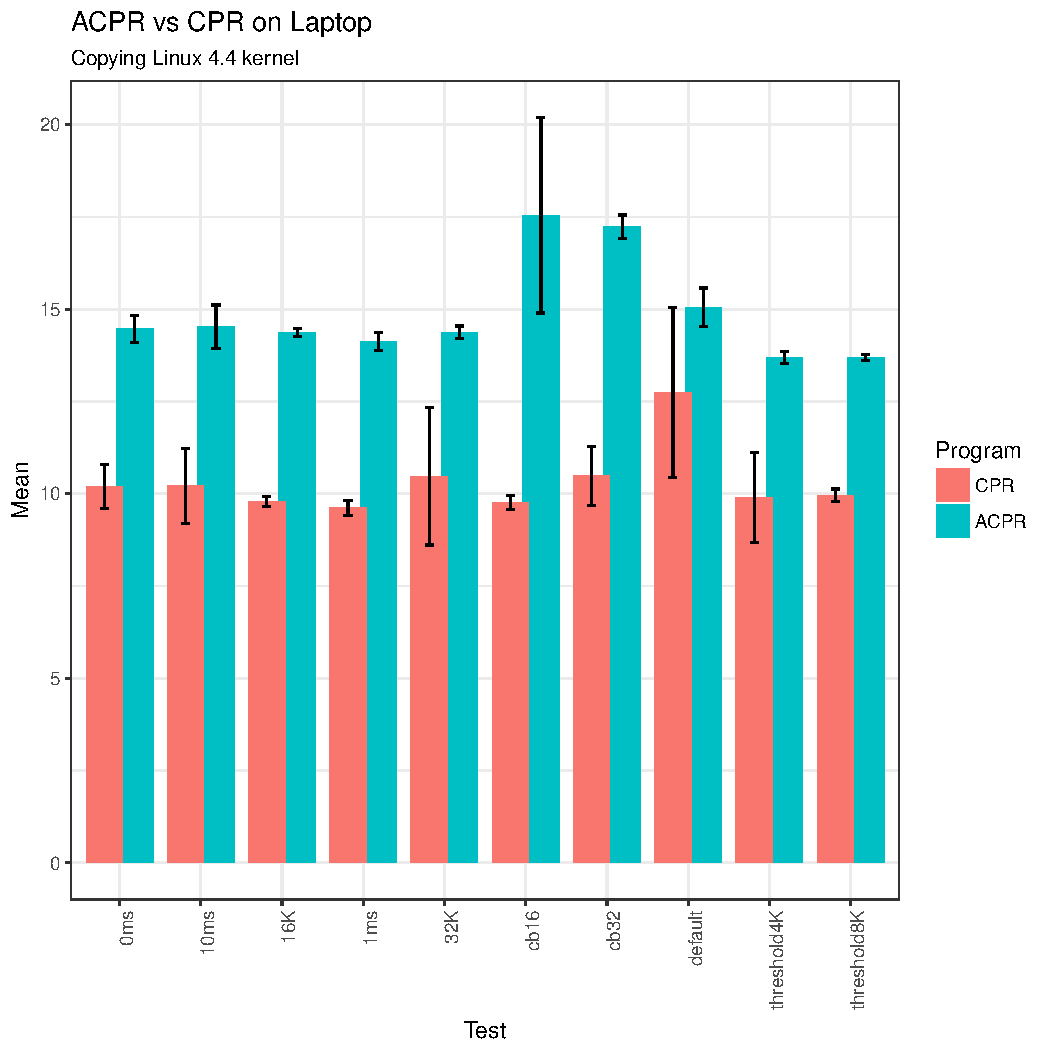
\includegraphics[width=1.8\textwidth,]{Laptop_Linux_Barplot.pdf}
                \caption{Copying Linux 4.4 on Thinkpad}
                \label{fig:laptop_linux}
        \end{minipage}
        \hspace{3cm}
        \begin{minipage}{.33\textwidth}
                \centering
                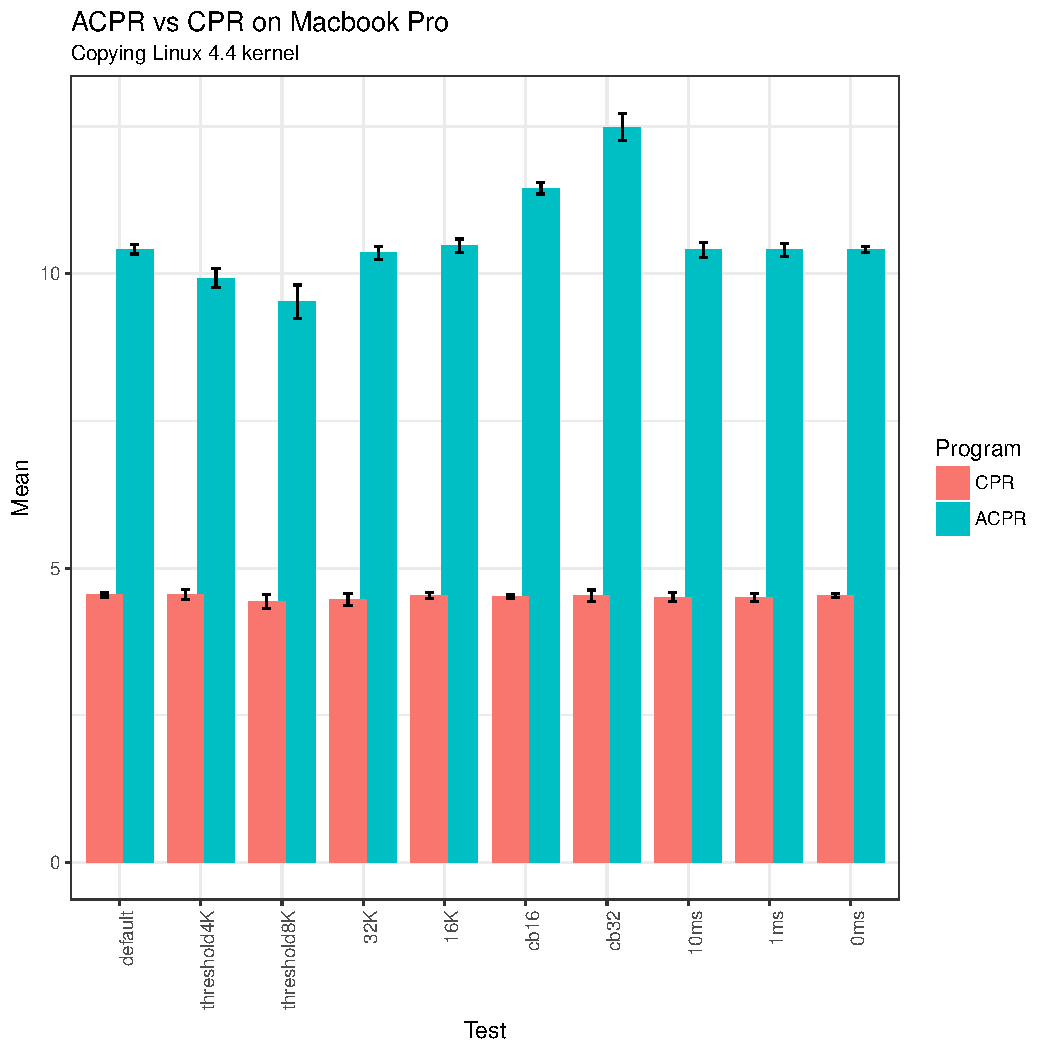
\includegraphics[width=1.8\textwidth,]{Macbook_Linux_Barplot.pdf}
                \caption{Copying Linux 4.4 on Macbook Pro}
                \label{fig:macbook_linux}
        \end{minipage}
\end{figure}

First, we compare a run of \texttt{acpr} with all default options vs. \texttt{cp
-r} on the Thinkpad. \texttt{cp -r} copies the 711 MB source tree in 12.75s for
46.48 MB/s throughput, while \texttt{acpr} manages 15.05s for 39.3 MB/s
throughput as seen in Figure~\ref{fig:laptop_linux}. On the Macbook Pro, we have
that \texttt{cp -r} copies the source tree in 4.5s with a throughput of 156 MB/s
as shown in Figure~\ref{fig:macbook_linux}. However, \texttt{acpr} copies the
source tree in 10.4s and throughput of 68 MB/s. Note how much lower this is than
copying a single file, since there is much more filesystem overhead to
\texttt{open}, \texttt{stat}, and \texttt{close} each individual file as opposed
to just one. 

The Linux source tree is composed of many different sizes of file. The default
threshold for \texttt{acpr} to use AIO is 1K, which may have too high of an
overhead. We instead tried raising the threshold for using AIO to 4K, which
would still copy 25984 files in the source tree using AIO. Doing this sped up
execution to 13.69s and 43.2 MB/s on the Thinkpad
(Figure~\ref{fig:laptop_linux}). Further raising the threshold to 8K does not
give a similar boost, remaining at 13.69s and 43.3 MB/s. For the Macbook Pro,
changing the threshold to 4k slightly increases performance to 9.9s and 71 MB/s
throughput while doubling the threshold to 8k results in another performance
increase to 9.5s and 74 MB/s. However, these numbers are still twice as slow as
the \texttt{cp -r} performance of 4.5s and 159 MB/s
(Figure~\ref{fig:macbook_linux}). This is as expected, since the number of files
larger than the threshold decreases drastically as the threshold increases.

The second experiment was to use a \textit{smaller} block size. Since many of
the files are source files that are a handful of KB large, the default block
size of 64K may have resulted in unnecessary overhead allocating space that ends
up going unused. Reducing the block size to 32K yields a small speedup to 14.37s
and 41.22 MB/s; reducing further to 16K does not produce further improvements,
staying at 14.37s and 41.25 MB/s, likely because the difference in overhead
becomes negligible on the Thinkpad (Figure~\ref{fig:laptop_linux}). On the
Macbook Pro, reducing the block size to 32k yields a similar negligible speedup to
10.35s and 68 MB/s. Going further to 16K actually decreases performance to
10.47s and 67 MB/s as seen in Figure~\ref{fig:macbook_linux}.

The third experiment was to vary the number of \texttt{iocb}'s used in copying
each file. The default is 5, and \texttt{acpr} waits until it has gathered 5
initialized \texttt{iocb}'s before it submits them to the kernel. So
theoretically, raising the number used should reduce the number of system calls
made, as they are batched together more. However, we saw reduced performance on
the Thinkpad - for 16 \texttt{iocb}'s per file, we got 17.54s and 33.79 MB/s;
for 32, we got 17.23s and 34.4 MB/s (Figure~\ref{fig:laptop_linux}). Similarly,
Figure~\ref{fig:macbook_linux} exhibits the reduced performance on the Macbook
Pro for 16 \texttt{iocb}'s (11.45s and 62 MB/s) as well as for 32 (12.49s and
56.9 MB/s). This is due to the large (64k or larger) buffers that must be
allocated and freed for each \texttt{iocb} of each copy task.

% TODO: Change laptop to Thinkpad in graphs

Our final experiment for the laptops was to vary the timeout when gathering
events. Changing the default of 5 ms to 10 ms on the Thinkpad gives a negligible
performance boost to 14.52s and 40.79 MB/s; lowering it to 1 ms does the same:
14.13s and 41.949 MB/s, as does eliminating the timeout completely: 14.46s and
40.97 MB/s (Figure~\ref{fig:laptop_linux}). By constrast,
Figure~\ref{fig:macbook_linux} demonstrates no significant change to the default
performance of 10.4s and 68 MB/s. Combined with the results from copying the
Lubuntu ISO, it seems that in the cases we have set up, the timeout passed to
the kernel when retrieving events does not matter, meaning that the kernel is
almost always ready with events for us to process. This potentially could matter
if we had extended \texttt{acpr} to use multiple threads for event processing.

\subsection{csres} \label{subsec:csres}

\begin{figure}[ht!]
        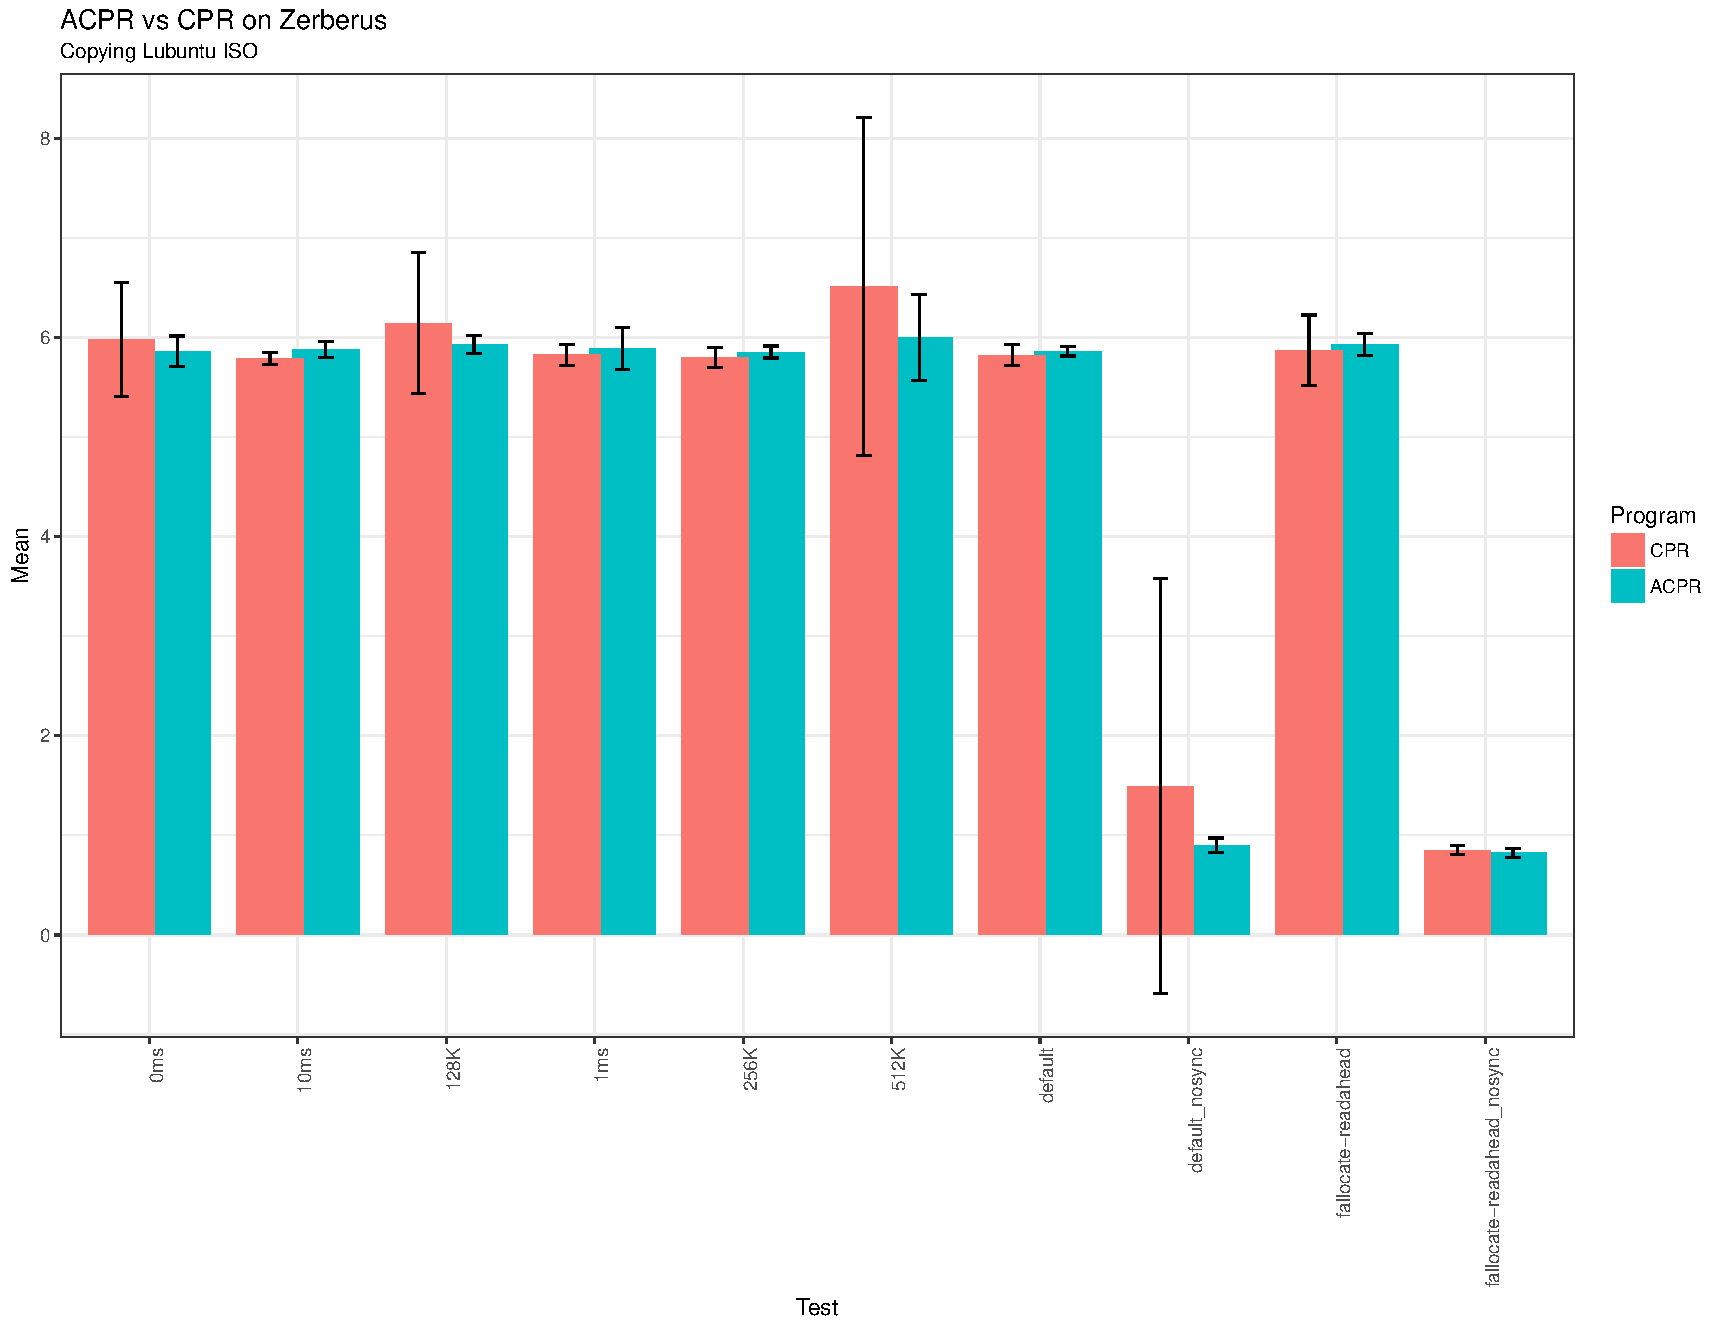
\includegraphics[width=\textwidth,]{CSRES_Lubuntu_Barplot.pdf}
        \caption{Copying Lubuntu on Zerberus}
        \label{fig:csres_lubuntu}
\end{figure}

The csres server machines run Ubuntu LTS 16.04.3, and have 32 Intel Xeon E5-2620
v4 processors clocked at 2.1 GHz, 126 GB of RAM, and 128 GB of swap space
configured. The tests were run on the \texttt{/var/tmp} directory, which is on a
local ext4 partition, instead of the NFS home directories. The partition is on a
Seagate 7200RPM enterprise-grade hard disk.

\subsubsection{Copying a Single Large File} \label{ssubsec:csres_large}

The same test cases as above were performed on
\texttt{zerberus.csres.utexas.edu}. Overall throughput was lower, as expected,
with the default configuration taking 5.86s and 150.18 MB/s. \texttt{cp -r}
barely did better at 5.82s and 151.15 MB/s (Figure~\ref{fig:csres_lubuntu}).

Employing \texttt{fallocate} and \texttt{readahead} actually slowed performance
down to 5.93s and 148.40 MB/s, though the difference is well within deviation.
For the rest of the experiments (adjusting the block size and timeout wait), the
results remained very close to the default configuration seen in
Figure~\ref{fig:csres_lubuntu}. We attribute this to a bottleneck that is
external to both \texttt{cp} and \texttt{acpr} - disk latency. 

To test this, we ran the baseline and \texttt{fallocate} cases again, without
the flag that calls \texttt{sync} and \texttt{echo 3 >
/proc/sys/vm/drop\_caches} every iteration. As expected, throughput was much
higher as our calls were now being serviced straight from memory. What was more
surprising, however, was that \texttt{acpr} had a clear speedup over \texttt{cp
-r} in both cases. In the default configuration with no syncing, \texttt{cp -r}
manages 1.49s and 589.59 MB/s while \texttt{acpr} finishes in 0.9s and 976 MB/s.
With \texttt{fallocate} and \texttt{readahead}, \texttt{cp -r} finishes in 0.85s
and 1033.97 MB/s and \texttt{acpr} in 0.82s and 1068 MB/s as seen in
Figure~\ref{fig:csres_lubuntu}. We attribute these results to the fact that the
AIO system now has the flexibility to schedule the disk reads and writes for
efficiency as well as the relatively large buffer cache on the csres machines.
We were unable to replicate similar results on our laptops, possibly due to
their smaller memories and the nature of SSD accesses.

\begin{figure}[ht!]
        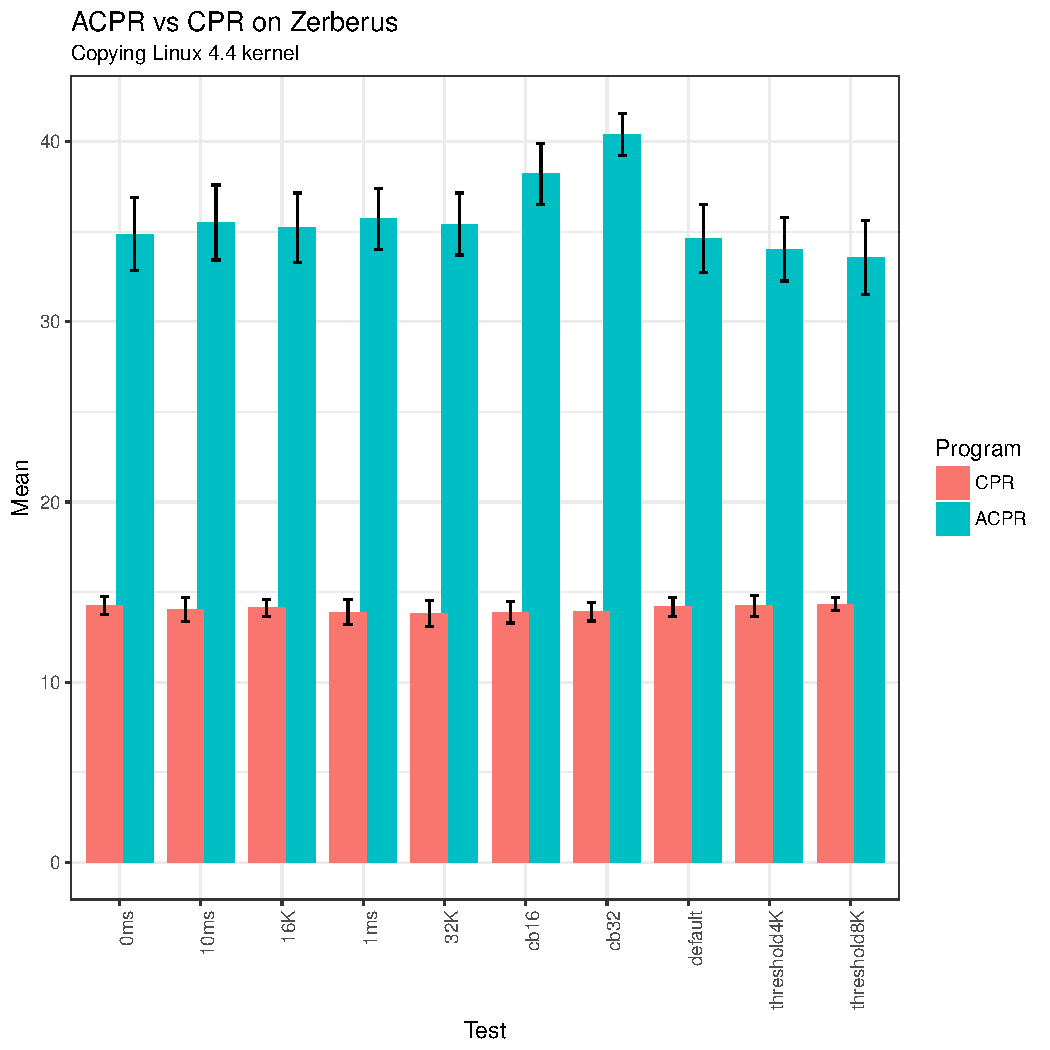
\includegraphics[width=\textwidth,]{CSRES_Linux_Barplot.pdf}
        \caption{Copying Linux 4.4 on Zerberus}
        \label{fig:csres_linux}
\end{figure}

\subsubsection{Copying Linux Source Tree} \label{ssubsec:csres_large}

Both \texttt{cp -r} and \texttt{acpr} performed quite poorly copying the Linux
4.4.97 kernel source tree, with \texttt{cp -r} taking 14.19s and 41.77 MB/s, and
\texttt{acpr} taking 34.6s and 17.11 MB/s. While increasing the threshold of
using AIO did improve performance, the change was miniscule. Likewise, for all
other cases (adjusting block size, adjusting \texttt{iocb} count, and adjusting
timeout), there was no significant change from the default configuration as
shown in Figure~\ref{fig:csres_linux}. Again, we attribute this to factors
beyond both programs' control. \texttt{acpr} is probably slower because the
kernel contains many small files, so the overhead of setting up AIO, allocating
buffers, etc.\ dominates the time to actually transfer the data.

\section{Conclusion} \label{sec:conc}

We have produced a prototype of a \texttt{cp -r} clone that uses Linux's
Asynchronous IO interface to perform its data transfers. While it does not
outperform \texttt{cp -r} except in two cases, it remains within acceptable
performance bounds, especially on SSD hardware. Further improvements would
include a more robust event handling system with multiple threads, support for
symbolic links, support for attribute copying, batching of write task
submissions, and a customized \texttt{copy\_file} implementation.

\section{Time Spent} \label{sec:time}

About 1.5 hours were spent researching the state of asynchronous IO, finding
documentation for the chosen libraries, and setting up the build system of the
project. About 8 hours were spent overall creating the acpr program itself,
including planning, programming, and optimization. About 10 hours were spent
creating the test harness, test cases, executing test cases, and collecting the
data. About 6 hours were spent creating the plots, report, and presentation. In total,
that is 25.5 hours spent on this project.

\begin{thebibliography}{99}
        \bibitem{aio7}
        aio (7), http://man7.org/linux/man-pages/man7/aio.7.html
        \bibitem{ubuntu}
        Asynchornous IO, http://manpages.ubuntu.com/manpages/precise/en/man3/io.3.html
        \bibitem{boost}
        Boost Source Control, https://github.com/boostorg/boost
\end{thebibliography}

\end{document}
